% Software Backend (Python)
% Zuständig: Jones

% wie/wo soll protobuf erklärt/erwähnt werden?

\chapter{Software - Backend}
\label{sec:software_backend}
\initials{JS}
Das Backend ist die zentrale Rechenstelle, 
welche in mehrere Komponenten aufgeteilt ist.
% generell zum backend

\begin{figure}[H]
    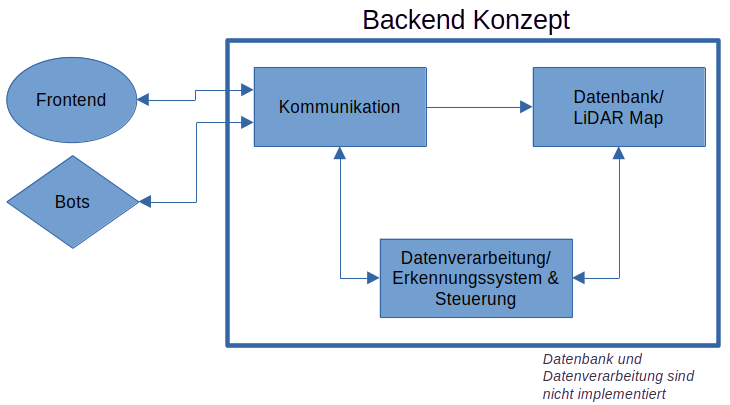
\includegraphics[width=\textwidth, center]{img/backend-konzept.png}
    \caption{Backend Konzept}
    \label{fig:backend_konzept}
\end{figure}
% grafik anpassen

Es ist verantwortlich für die Kommunikation und Datenerfassung 
zwischen allen Teilnehmern. 
Dazu gehören die drei Roboter, welche die Daten liefern wie LiDAR, 
Beschleunigungssensor etc., und das Frontend, 
zu dem die Daten zur Visualisierung und Mitverfolgung gesendet werden 
und von dem gegebenenfalls auch Befehle empfangen werden.
\\
Weiters findet hier die zentrale Datenverarbeitung und Verwaltung statt, 
diese ist verantwortlich für die Erstellung der LiDAR-Map, 
die Ermittlung der Roboterpositionen und gegebenenfalls die Berechnung der Messwerte. 
% im falle ineffizient etc
\\
Eine weitere Aufgabe des Backends 
ist die Steuerung der Roboter mithilfe eines Erkennungssystems, 
welches nach bestimmten Kennzeichen in den erhaltenen Daten Ausschau hält 
und darauf Kennzeichen für die einzelnen Bots erkennt und verfolgt, 
um entsprechend die Positionen aller Bots relativ zur LiDAR-Map ausfindig zu machen.
% 
% Die Zentrale Datenverarbeitung und autonome Steuerung der Roboter sind 
% im zu zeitigen Prototypen stand nicht implementiert.
% % stattdessen weiterleitung und fernsteuerung
% TODO 
\\
Letztendlich verwaltet das Backend die Datenbank, 
welche die etwaigen Daten der Datenverarbeitung und des Erkennungssystems speichert, 
dazu gehört insbesondere die LiDAR-Map.

Für die Programmierung des Backends wurde die Sprache Python gewählt, 
welche mit ihrer Vielzahl von Standardpaketen 
und großen Anzahl an externen Paketen 
und Frameworks eine effiziente und schnelle Programmierung unterstützt, 
auch durch eine aktive Community.
% 
Für dieses Projekt wurde es gewählt aufgrund seiner Vielseitigkeit, 
speziell in Bezug auf die unterschiedlichen Tasks, 
die ausgeführt werden müssen, 
hauptsächlich in Bezug auf Kommunikation und Datenverarbeitung, 
in denen Python üblicherweise verwendet wird.
% 
Dabei müssen auch mehrere Verbindungen offen bleiben und verwaltet werden, 
und diese wesentlichen Eigenschaften für einen Server 
schnell mithilfe von Paketen realisiert wurde. 
% 
Die uns ermöglichen, aufs wesentliche zu fokussieren.
% 
Effiziente Programmierung und Modifizierung ist wesentlich, 
weil der Backend-Code kontinuierlich wächst.
% 
Dies wurde auch durch Erfahrungen mit dem Vorgänger-Projekt untermauert, 
denn ein wesentlicher Teil davon bestand aus der Kommunikation über Websockets.
% Gelaber über python
% wegen math Funktionen...
% schnelle Modifizierung 
% packet/ Bibliothek Fokussierung auf Einfachheit
\section{Systembeschreibung}
\initials{JS}
% drunter verschoben weil besseres layout?
In diesem Abschnitt wird genauer 
über die geplanten einzelnen Komponenten 
und deren Funktion gesprochen.

Zu beachten ist, dass nicht alle geplanten Systeme, die hier beschrieben sind, 
implementiert wurden und manche noch in der Konzeptphase sind.
Für den tatsächlichen Stand siehe Abschnitt \ref{subsec:backend_aktueller_stand}.

\subsection{Datenverwaltung}
\label{subsec:backend_data}
\initials{JS}
% übersicht über die drei komponenten und wie ungefähr der datenfluss aussieht?
% TODO
% Datenbank für lidar?
% TODO

% TODO bevor abgabe
% womöglich löschen
Dieser Abschnitt bespricht kurz den Datenablauf 
zwischen den Teilnehmern und den internen Komponenten.
% 
Weil teile des Backends nicht realisiert sind ist ebenfalls 
die Datenverarbeitung nicht realisiert,
weswegen nicht viel weiter zur Verwaltung gesprochen werden kann.

\subsection{Kommunikation}
\label{subsec:Kommunikation}
\initials{JS}
Die drei Roboter sind aktive Teilnehmer in der Kommunikation, 
das heißt, die Verbindung ist permanent aufrechtzuerhalten, 
bidirektional und zeitlich synchronisiert. 

Zur Verbindung entschieden wir uns für das Kommunikations-Protokoll Websocket, 
dieses ermöglicht eine bidirektionale, 
persistente Verbindung zwischen Client und Server,
welche im Vergleich zu gewöhnlichen HTTP-Anfragen offen bleibt, 
wodurch Echtzeitkommunikation möglich ist.
% könnte man mehr ausschreiben aber schau ma später

Das Frontend und die Roboter kommunizieren hauptsächlich 
über Websockets mit den Protobufs.

\subsection{Datenverarbeitung}
\initials{JS}
% TODO
Eine Aufgabe des Servers ist die Verarbeitung der erhaltenen Daten, 
sowie die Weiterleitung zum Frontend.
% 
Um große Belastung durch die Auswertung von Sensordaten auf dem Roboter zu vermeiden, 
werden einige Arbeiten auf den Server ausgelagert.
Außerdem stehen in Python bereits ausgebaute Mathematik Pakete zur Verfügung 
um die Sensordaten zu bearbeiten 
ebenso wie Softwarepakete für Datenanalyse und -manipulation.


\subsection{Erkennungssystem}
\initials{JS}
Geplant war, dass aus den erhaltenen Daten mit der Zeit eine Karte erstellt wird, 
sozusagen die LiDAR-Map, 
welche in einer Datenbank abgespeichert wird.
% 
Über die Zeit werden Datenpunkte gesammelt, 
die sich nach einem gewissen Muster sammeln 
und ein klareres Bild über die Form eines Raumes geben.
Diese Muster, z.B. gerade Linien und Ecken, werden vom System erkannt 
und mit diesen Eigenschaften auch ermittelt, 
wo ungefähr sich der Guide im Raum befindet.
% 
Dies wird mit einem weiteren Erkennungssystem für Tamerlan \& Bambi kombiniert, 
welches zuständig ist, die Position der beiden zu ermitteln,
indem auf den Bots identifizierbare reflektieren Objekte befestigt werden, 
beispielsweise Zylinder, wodurch sie erkannt werden können.
%
Mit diesen Informationen kann die Steuerung der Roboter folgen.
% füge skizzen hier oder erklär anderen Kapitel?
% Kugel, stab, mehrere stäbe, reflektierendes material

Eine genauere Beschreibung der LiDAR Karte und wie diese aussieht, 
ist im Frontend Abschnitt \ref{subsec:frontend_lidar_map} 
auf Seite \pageref{subsec:frontend_lidar_map} zu finden.

\subsection{Steuerung der Roboter}
\label{subsec:backend_robot_detection}
\initials{JS}
% TODO
Zurzeit nicht realisiert.
% spätester schritt weil funktionierende Strategie benötigt wird zur Erkennung
% Datenbank/ Datenbearbeitung

Die Aufträge der einzelnen Bots 
sind in den entsprechenden Kapiteln genauer beschrieben.
% schau was da steht und was speziell hier klargemacht werden muss

Es sind zwei Steuerungen geplant, 
die manuelle Steuerung und die automatisierte.
% 
Die manuelle Steuerung geschieht über das Frontend, 
womit man die Roboter mithilfe der Visualisierungen 
und oder Videoübertragung steuern kann.
% 
Die automatisierte Steuerung geschieht mithilfe des Erkennungssystems 
und soll den Bots erlauben, die erstellte LiDAR Karte zu navigieren 
und erlauben den zwei blinden Bots Tamerlan \& Bambi, dem Guide zu folgen.
% verwendung von code vom vorgänger Projekt

\section{Aktueller Stand}
\label{subsec:backend_aktueller_stand}
\initials{JS}

\begin{figure}[H]
    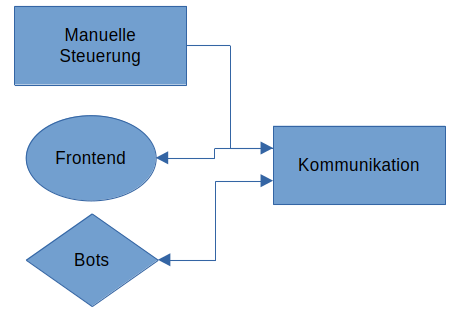
\includegraphics[width=0.7\textwidth, center]{img/Backend/backend-aktuell.png}
    \caption{Backend Aktuell}
    \label{fig:backend_konzept}
\end{figure}

% Womöglich Teile zu Ergebnisse verschieben?
Zum Zeitpunkt dieser Diplomarbeitsabgabe 
sind nicht alle geplanten Features für das Backend implementiert,
Wodurch der Großteil der Backendserver-Seite nicht realisiert werden konnte.

Zur Überbrückung wurde der Kommunikationsteil so realisiert, 
dass es als Weitergabe fungiert.
Dies wurde so realisiert, dass die Daten 
zwischen einem Bot und dem Server weitergegeben werden, essenziell ein Router. 
Der nächste Schritt besteht dann, über eine Prototyp Steuerung 
Befehle zu den einzelnen Bots zu senden.

Die Prototyp Steuerung ist realisiert als eine manuelle Steuerung, 
wo der gewählte Roboter manuell von einem User bedient wird.
In Zukunft kann die manuelle Steuerung als eine weitere Option beibehalten werden, 
die die automatisierte Steuerung überschreiben kann. 
Dies kann verwendet werden, 
um beispielsweise den Guide manuell in bestimmte Bereiche zu führen,
andernfalls auch für Test und Debugging, 
sowie um eine neue Datenerfassung zu erzwingen.

\section{Backend - Code}
\initials{JS}
In diesem Abschnitt wird genauer auf den Code des Backend Prototyps eingegangen 
und auf dessen technische Realisierung. 
Weiters wird auch beschrieben, welche Pakete und Werkzeuge verwendet wurden. 

\subsection{Zusätzlich verwendete Tools und Workflow}
\initials{JS}
% algemein zu python workflow
% womöglich unötig
% TODO
\subsubsection{Formatter und Linter} 
\initials{JS}
Um gute Lesbarkeit zu gewährleisten, 
ist eine ordentliche Struktur und Formatierung in jedem Code notwendig, 
jedoch ist es schwierig, eine gute Konsistenz beizubehalten, 
weshalb Formatierungstools und Linters häufig Verwendung finden. 
% 
Linters sind Tools, welche automatisch den Code überprüfen, 
um stilistische Fehler und Einhaltung von Codierung Standards sicherzustellen.
Dies soll helfen, die Code-Qualität zu verbessern 
und eventuelle Fehler frühzeitig zu erkennen.

Die Standard-Erweiterung für Python von Visual Studio Code 
beinhaltet kein Formatierungstool.
Dafür wurde der Formatter \texttt{autopep8} verwendet, 
weil er die Eigenschaft hat, den Originalstil des Schreibers beizubehalten
und nur Änderungen für die Lesbarkeit durchzuführen. 
Dazu passend ist der Linter \texttt{Flake8}, welcher standardmäßig 
dem gleichen Styleguide \text{PEP 8} folgt.
% weil vscode es standart mäßig Formatierung nicht mitliefert
% \subsubsection{venv/environment management}
% \initials{JS}
% % TODO
% Falls sich nicht viel ändert, ist dieser Abschnitt wahrscheinlich nicht nötig, 
% da nicht viel besonders ist.


\subsection{Python Packages}
\initials{JS}
% TODO schau dir dieses abschniit nochmal durch
Um gegebene Funktionen zu gewährleisten, sind weitere externe Pakete nötig, 
die nicht Teil der Standardpakete sind.
Welche zu diesem Stand verwendet wurden, ist in diesem Abschnitt erklärt.

\subsubsection{websockets}
\initials{JS}
Für Python ist ein Websocket Paket namens 'websockets' vorhanden, 
welches die Client-Server Kommunikation um ein Vielfaches vereinfacht, 
da man sich keine Sorge über Handshakes, Ping Pongs, 
oder anderes Verhalten der Websocket Spezifikation machen muss, 
da es alles von dem Paket behandelt wird 
und man sich mehr auf die Applikation fokussieren kann. 
Es sind dennoch einige Parameter zur Verfügung gestellt, 
um das Verhalten zu modifizieren.
% code beispiele?

% erklärung zu den packet Webscoket
Websockets Standard Implementierung basiert auf asyncio.
%  
Asyncio ist die eingebaute Implementierung von Co-Routinen in Python,
dies erlaubt das Schreiben von asynchronen Frameworks, 
öfters verwendet für I/O-limitierte Netzwerk Codes.
% snippet zu asyncio, könnte mehr schreiben?
Alternative ist eine threading Implementierung verfügbar für Websockets, 
die üblichere Implementierung von mehreren Tasks, 
jedoch wurde für den derzeitigen Entwicklung-Stand dagegen entschieden,
aufgrund der möglichen erweiterten Komplexität von Thread-sicherer Code-Ausführung.
% warum nicht? kann später bei optimierungsmöglichkeiten erklärt werden
Eine Sans-I/O Implementierung ist auch vorhanden, 
jedoch für dieses Projekt zurzeit irrelevant.

\subsubsection{protobuf}
\initials{JS}
Das Besondere an der protobuf Implementierung hier in Python ist,
dass sehr viel von dem protobuf Paket selbst erledigt wird.
Im Vergleich zum Vorgänger Projekt, wo die Datenpakete manuell hergerichtet werden
und zum richtigen Byte Format konvertiert werden mussten, 
wird mit Protobuf ein Objekt erstellt 
und jeweils die gegebenen Variablen angesprochen, 
diese mit einem einzelnen Befehl ins Sende-Format konvertiert und umgekehrt.
% verhalten in python
% wie anders

% Kurzeitig gab es das Problem wie genau mit dem protobuf paket zu arbeiten ist,
% aufgrund dessen das die dokumentation nicht der von anderen Python Paketen gleicht
% und alle Informationen hauptsächlich von der Anleitungen zu Wünschen übrig lässt.
% Ich hatte einfach ein wenig probleme es anfänglich zu kapieren aber ging schnell

\subsubsection{pygame}
\initials{JS}
Dieses Paket wird ausschließlich für die manuelle Steuerung verwendet.
Hauptsächlich wird es zum Entwickeln von Spielen in Python genutzt,
doch in diesem Projekt dient es der einfachen Konfiguration von Controllern.

\subsection{Kommunikation - test\_server\_passby.py}
\initials{JS}
In diesem Abschnitt wird über die Kommunikation 
und bestimmte technischen Implementierungen angesprochen.

Der Prototyp hat die Funktion, zwei Typen von Verbindungen zu bearbeiten: \\
%
1. Die der Bots, welche als Server agieren; 
das bedeutet, 
dass sich dieser Backend-Server mit den drei Robotern verbinden muss, 
während das Frontend standardmäßig als Client fungiert. 
Das heißt, dass die Clients eine Verbindung mit dem Backend Server herstellen. \\
% 
2. Die Verbindung mit dem Frontend, 
welche vom Server für einkommende Verbindungen bereitgestellt werden muss.
% 
Die Daten, die von der jeweiligen Seite kommen, 
werden zurzeit zur anderen Stelle weitergeleitet.

Dementsprechend ist die Kommunikation auf zwei Tasks aufgeteilt,
die des Frontends und die der Roboter.
% 
Beide Tasks starten einen weiteren Subtask, welcher nebenbei laufen wird, 
dieser hat entsprechend die Aufgabe, 
solange die Websocket Verbindung offen ist,
die ankommenden Pakete zu erwarten 
und diese entsprechend in eine Queue Puffer abzulegen, 
um weiter verarbeitet zu werden. 

Beide Tasks verarbeiten die Queues, 
in denen eine bestimmte Anzahl der Elemente im Puffer 
einzeln geholt und die Protobuf Wrapper verarbeitet werden.
% 
Im derzeitigen Prototyp werden die Daten in die Konsole ausgegeben,
und zur Sendung der Gegenseite in eine weitere Queue 
für einen beliebigen Roboter bereitgestellt, 
oder im Code des derzeitigen Roboter-Handler 
an alle verbundenen Frontends gesendet.
% 
Dies ist eine Vorbereitung auf die nächsten Iterationen 
(Weitergabe in die Datenbank und Datenverarbeitung).

% übersichtsgrafik über teilnehmer und wie datenablauf funktioniert
% asyncio - warum
% main task überblick (server und drei clients) warum so aufgeteilt?
% subtask

\subsubsection{asyncio}
\initials{JS}
% erklärung zu asyncio
Um mehrere separate Tasks auszuführen, wurde asyncio,
die eingebaute Implementierung von Koroutinen in Python, verwendet.
% 
Asyncio funktioniert, 
indem Tasks sich die gleiche CPU-Zeit teilen über den Event Loop,
dies geschieht, indem sie mit dem 'await' Befehl freiwillig die Kontrolle abgeben,
wenn sie auf etwas warten, z.B. dass Daten vom Websocket ankommen.
Während dessen wird der Event Loop andere Task durchführen, 
solange der erste Task wartet.

Im Gegensatz zu üblichem Multitasking,
wo jeder Task eine feste Zeit vom Betriebssystem zugeschrieben bekommt, 
und es entscheidet, wenn ein Task an der Reihe ist.
% 
Der Größte Unterschied jedoch ist das asyncio Tasks sich alle einen Thread teilen,
dies bedeutet das Asyncio Programme auf einen einzelnen Kern limitiert sind.
% 
Während threading z.B. viel mehr CPU-Overhead besitzt, 
weil es auf mehreren Threads laufen kann, 
bringt es auch eigene Herausforderungen mit.
% 
Davon können wir jedoch bei derzeit nur 4 Teilnehmern nicht profitieren.
Deshalb haben wir uns für die Effizienz und Skalierbarkeit von asyncio entschieden.

% TODO Womöglich weiter beschreiben, wie asyncio genau funktioniert?
% Frag ob das so passt jetzt?

\subsubsection{Queue Buffers}
\initials{JS}
% FIFO Queues
% Wichtigkeit nicht blockierendes verhalten um asynchrones workflow zu gewährleisten
Damit keine Nachrichten verloren gehen, 
weil die adressierten Prozesse gerade nicht aktiv sind,  
wird der Empfang von Websockets abgekoppelt von der Backend-Logik.
Dafür werden Queues, realisiert als FIFO, verwendet, also ein Zwischenspeicher, 
wo die erhaltenen Daten von den Websockets landen, 
um dann später weiterverarbeitet zu werden.
% 
Somit können wir einen Prozess starten, 
welcher auf eingehende Nachrichten warten kann,
während unser Backend andere Prozesse ausführt.
% kann mehr dazu schreiben
% ermöglicht auch sachen etc.
% TODO

\subsection{Prototyp manuelle Steuerung}
\initials{JS}
Die Steuerung soll einem Bediener erlauben, manuell die Bots zu steuern. 
% 
Dafür verwenden wir einen Controller, 
weil wir bereits im Vorgängerprojekt
eine solche Steuerung realisiert haben. 
Deshalb ist ein Großteil der Arbeit hier die Anpassung an das neue Datenformat, 
Verwendung neuer Websocket Pakete und Modifizierung der Berechnungen.
% 
Es ist geplant, dies zuerst als einzelnes Skript zu realisieren, 
welches den Platz des Frontends einnimmt, 
um im Laufe des Projekts ins Frontend integriert oder neu implementiert wird.

% TODO aktualisiere dies entsprechend
% TODO
\subsubsection{Controller Steuerung}
\initials{JS}
Dafür wird das Paket pygame verwendet,
das für die Verbindung mit den Controllern verantwortlich ist,
unabhängig davon, ob sie verkabelt oder über Bluetooth verbunden sind.

\subsubsection{Begrenzung Änderungsrate}
\initials{JS}
Ein zusätzlicher Teil der Steuerung ist die Begrenzung der Änderungsrate, 
die unabhängig von der Laufzeit des Codes arbeitet.
% 
Diese wurde implementiert, weil zu starke Sprünge der Werte in der Motorsteuerung 
im Vorgängerprojekt die Motorsteuerung überlasteten.
% 
Im aktuellen Projekt sorgt sie nun für ein sanfteres Verhalten für den Benutzer 
und eine bessere Balancierung.
\begin{lstlisting}[language=python, gobble=4]
    max_expected_change = int(2147483647*0.75)  # per second based on +-

    def change_dampening(current_value, past_value,
                     current_time, past_time,
                     max_expected_change):
    # used for limiting the maximum rate of change in the detected time window
    delta_t = current_time - past_time

    relativevalue_change = (current_value - past_value)/(delta_t)
    relativeexpected_change = (max_expected_change/(delta_t))

    if (relativevalue_change) > relativeexpected_change:
        # catches exceeded positive change
        past_value = past_value + relativeexpected_change * delta_t
        past_time = current_time
    elif (relativevalue_change) < -relativeexpected_change:
        # catches exceeded negative change
        past_value = past_value - relativeexpected_change * delta_t
        past_time = current_time
    else:
        # passes value through
        past_value = current_value

    return past_value, past_time
\end{lstlisting}

\subsection{Konsolen Ausgabe}
\initials{JS}
% siehe print_wrapper_content.py
Der Skript \texttt{print\_wrapper\_content.py} hat die simple Funktion, 
die Daten von einem Protobuf Wrapper in die Konsole auszugeben, 
in einer für User lesbaren Struktur. 
Hauptsächlich genutzt für Debug und Entwicklungsschritte.

\begin{figure}[H]
    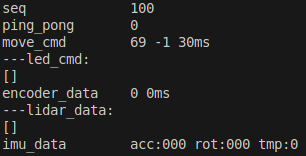
\includegraphics[width=0.5\textwidth, center]{img/Backend/print_wrapper_all.png}
    \caption{Python - Protobuf Konsolenausgabe}
    \label{fig:py_konsole_o}
\end{figure}

In Zukunft kann dies durch die Datenbank oder ein CSV Log abgelöst werden.
% 
Diese könnten automatisch nach Auffälligkeiten suchen 
und entsprechend melden und in einem Log abspeichern.

% \section{Protobuf Generierung}
% \initials{JS}
% % TODO
% Zurzeit nicht implementiert.

% Ein kleines Skript, welcher die Protobuff Dateien generiert
% und die Imports richtig setzt. 

% \section{Konfiguration Datei}
% \initials{JS}
% % TODO 
% Zurzeit nicht implementiert.

% Bestimmte Konfigurationen wie die Roboter Adressen 
% sollten in einer eigenen Konfigurations Datei landen und nicht im Code gesetzt sein.


\subsection{Optimierungsmöglichkeiten}
\initials{JS}
\label{subsec:Optimierungsmöglichkeiten}
\subsubsection{uvloop - schnellere Koroutinen}
\initials{JS}
% uvloop - drop in replacement
% https://github.com/MagicStack/uvloop
uvloop ist ein schneller Drop-in-Ersatz für die in asyncio integrierte Event-Loop. 
Dieser ist entsprechend in Cython entwickelt 
(Cython ist eigentlich Python, aber als Performanten C code compiliert).
Ziel dieser Ersetzung ist es, asyncio um einiges schneller zu machen, 
aber nicht von dem in asyncio gegebenen Verhalten abzuweichen. 
Als drop-in Ersatz geht dies so weit, 
dass die Abweichungen als Fehler kategorisiert werden.
% 
Während der Prototyp Phase dieses Projekts 
sind wir bei der Standard Implementierung geblieben, 
weil wir erst später im Projekt von uvloop erfahren haben.
In Zukunft wird jedoch eine Implementierung in Betracht gezogen,
aufgrund der vorhin genannten Eigenschaften,
insbesondere, wenn die nachfolgenden Projekte weiter skalieren.

% compelierung python code
\subsubsection{Kompilierung}
\initials{JS}
Es ist möglich, Python Code genauso wie jedes andere Programm zu kompilieren,
jedoch ist dies standardmäßig nicht nötig, 
da der Interpreter CPython (die Implementierung von der Python Programmiersprache) 
automatisch Python quell code zu byte code kompiliert (in PYC Dateien).
Das prekompilieren wird hauptsächlich dafür verwendet, 
um die Startzeit zu verringern 
und um den Code für die gewählte Platform einfacher zu verteilen,
weil man keine weiteren Pakete installieren muss, 
sondern nur die PYC Datei allein genügt.
% Dies ist jedoch für dieses Projekt irrelevant.

% \subsection{threading vs asyncio}
% \initials{JS}
% % TODO threading warum nicht streng nötig 
% % (hauptsächlich limitiert über Wifi I/O nicht anzahl an geräten & )
% % falls anzahl größer wird dann villeicht
% Eine andere Option um separate Task auszuführen ist die threading Implementierung.
% Diese erlaubt, dass ein Programm auf mehreren Threads ausgeführt werden kann. 

\section{Probleme}
\initials{JS}
\subsection{Linux Modifikationen}
\initials{JS}
Es kam das Problem auf, 
dass die lokale IP-Suche auf Linux Ubuntu nicht funktioniert.
Dies lag daran, 
dass die vorherige Variante mithilfe des Domain-Namens die lokale IP-Adresse findet.
In Linux wird jedoch eine andere Adresse zurückgeliefert, 
und zwar die Loopback-Adresse \texttt{127.0.1.1}. 
Diese Adresse wird verwendet, um dem \texttt{host\_name} eine Adresse zuzuweisen,
im Falle, dass kein Netzwerk vorhanden ist. 
Sonst kann eine permanente IP-Adresse hier zugewiesen werden.
% https://askubuntu.com/questions/754213
% /what-is-difference-between-localhost-address-127-0-0-1-and-127-0-1-1

Als Lösung öffnet das Programm temporär ein Socket 
und findet mit diesem die lokale IP-Adresse, wodurch es plattformunabhängig wird.
\begin{lstlisting}[language=python, gobble=4]
    import socket

    def get_local_ip():
    """
    opens a temporary socket connection and retrieves the local IP
    """
    s = socket.socket(socket.AF_INET, socket.SOCK_DGRAM)
    try:
        # doesn't even have to be reachable
        s.connect(('10.255.255.255', 1))
        IP = str(s.getsockname()[0])
    except Exception as b:
        print("error at figuring out local ip")
        print(b)
        exit
    finally:
        s.close()
    return IP
\end{lstlisting}

\subsection{Potenzielles blockierendes Verhalten}
\initials{JS}
% bot_handler und server nicht separat gestartet werden.
Obwohl die Kommunikation in zwei Teile aufgeteilt ist, 
mit Bot-Handler und Server, 
jedoch werden sie zu diesem Zeitpunkt gesammelt und gemeinsam gestartet.
Dies führt zu einer ungewollten Konsequenz,
dass, falls der Bot-Handler sich frühzeitig oder ungewollt beendet, 
nicht neu gestartet wird, bis sich ein neuer Client verbindet.
% 
Da jedoch für diese Diplomarbeit zu erwarten ist, 
dass die Bots stets zur Verfügung stehen sollten,
wird der Prozess, bei einer geschlossenen Verbindung für eine gewisse Zeit pausiert,
bevor ein neuer Verbindungsversuch gestartet wird.

In den nächsten Iterationen sollten jedoch 
die zwei Aufträge unabhängig gestartet werden können, 
um zu vermeiden, 
dass die ganze Kommunikation neu gestartet werden muss.

\subsection{Protobuf Generierung}
\initials{JS}
% siehe server/README.md
% verlege zu Backend probleme?
Während der Migration vom Vorentwicklungsordner, 
wurde für eine gewisse Zeit in einem Testordner experimentiert.
Dies führte dazu, dass der generierte Protobuf-Code nicht funktionierte,
da der Wrapper nicht über den Unterordner Standort \text{protobuf} 
der weiteren Protobuf-Dateien informiert wurde,
da das Kompilieren der Protobuf-Dateien für Python unabhängig vom Standort
der Python Umgebung geschieht, 
wodurch die Importe im generierten \text{wrapper\_pb2.py}
mit dem Ordner vorangestellt werden müssen.

\begin{lstlisting}[language=python, gobble=4]
    import protobuf.move_cmd_pb2 as move__cmd__pb2
    import protobuf.led_cmd_pb2 as led__cmd__pb2
    import protobuf.lidar_data_pb2 as lidar__data__pb2
    import protobuf.encoder_data_pb2 as encoder__data__pb2
    import protobuf.imu_data_pb2 as imu__data__pb2
\end{lstlisting}


\section{Test Codes}
\initials{JS}
Es wurde auch Testcode geschrieben, 
um die Kommunikationskanäle und Datenbearbeitung innerhalb 
und außerhalb des Backends zu testen und gegebenenfalls 
von anderen Teammitgliedern modifiziert zu werden.
% 
Aber auch für die Fehlersuche ist Testcode eine schnelle Option, 
um die Kommunikation und Datentausch zu testen.

Dieser Code hat große Ähnlichkeiten mit der Prototyp Kommunikation, 
deshalb wird in diesem Abschnitt hauptsächlich auf deren Nutzen eingegangen.

\subsection{Einzelverbindung - Robot\_ws\_test.py}
\initials{JS}
Dieser Testcode ist verantwortlich, sich mit den Bots zu verbinden 
und dessen Daten zu lesen.
Er wurde mit einigen Konfigurationen erweitert und modifiziert 
und wird im Laufe des Projekts angepasst.
Zurzeit wurde es bereits verwendet, 
um die Kommunikation zu testen 
für die Bearbeitung von erhaltenen Daten vom Bot 
und für generelle Fehlersuche.

\subsection{Client und Server}
\initials{JS}
Dazu gehören \texttt{test\_wrap\_client.py} (als das Frontend) 
und \texttt{test\_wrap\_bot\_transceiver.py} (als die Bots).
Dies ist einfacher Code, welcher Client und Server (Bots und Server) emuliert, 
indem sich beide Protobuf Pakete zuschicken. 
Dieser Code dient hauptsächlich dem Testen der Websocket-Kommunikation 
und auch zur Übung, wie Protobuf in Python zu verwenden ist, 
und nimmt die Position des Frontends und Bots ein.
Die zwei Senden und Empfangen die Protobuf Wrapper über die Backend Kommunikation 
und geben diese in die Konsole aus.
